\chapter{\glsentrylong{TCP}/\glsentrylong{IP} (\glsentryshort{TCP}/\glsentryshort{IP})}

\section{\gls{TCP}}
\begin{itemize}
\item It is the core protocol of the Internet that provides
  \popup{reliable}{Ordered and error-free.}, data delivery between
  \popup{networked entities}{Computer applications, ...}
  \cite{wikipedia_TCP}.
\item Bidirectional communication: Both entities can send and receive
  data during a given interval or time.
\end{itemize}

\section{Steps and timings}
\begin{itemize} 
\item The entities must follow a sequence of steps and waitings to ensure the communication.
\begin{figure}[H]
  \vspace{-0ex}
  \centering
  \href{https://www.ibm.com/support/pages/flowchart-tcp-connections-and-their-definition}{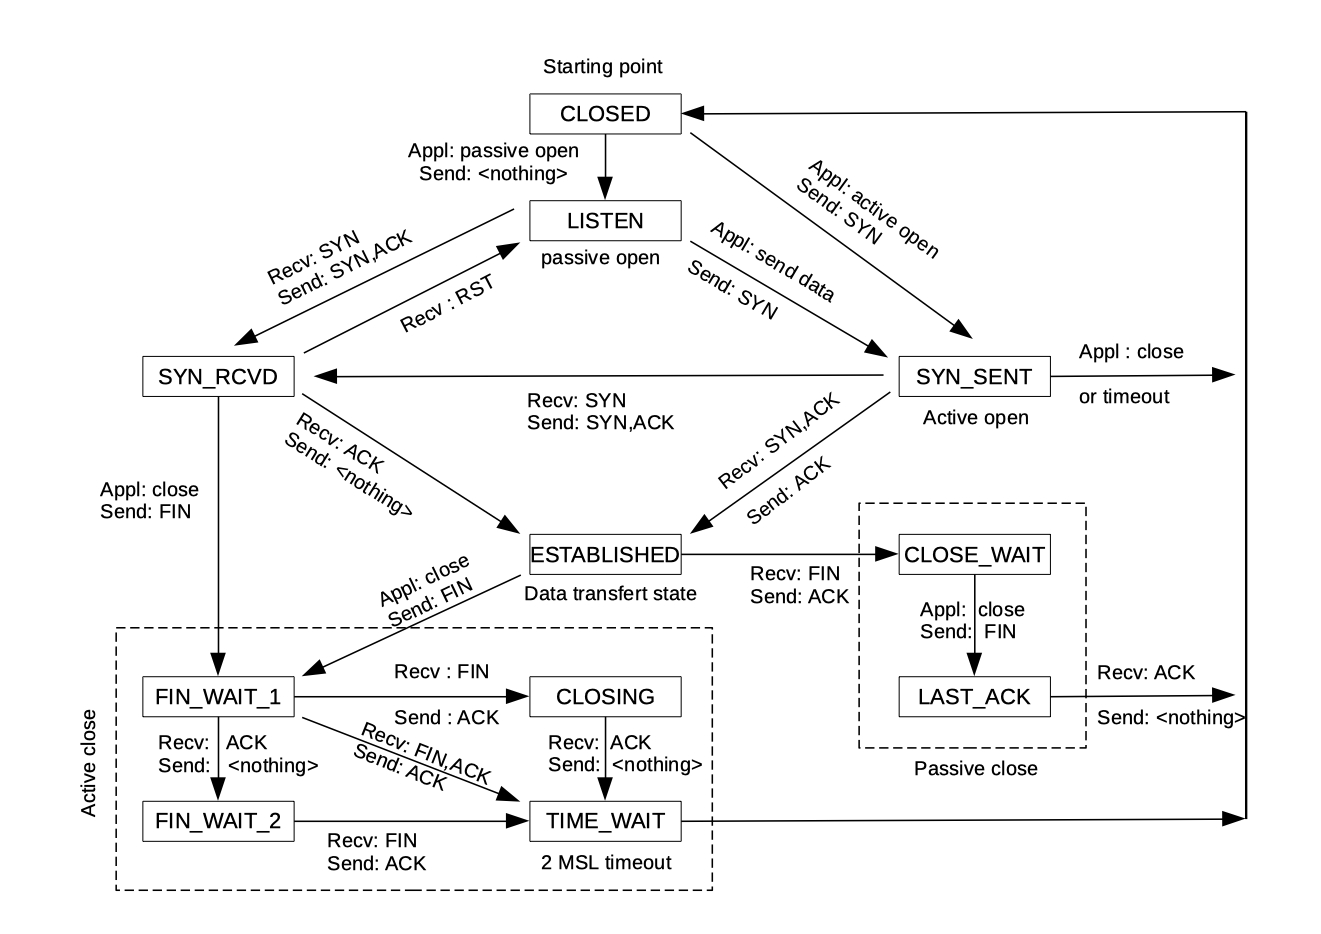
\includegraphics[height=5.5cm]{Flowchart_TCP}}
  \caption{States (and how are the transition between them) of the
    entities that use the \gls{TCP}.}
  \label{fig:TCP_states}
\end{figure}
\end{itemize}


\section{Transmission control}
\begin{itemize} 
\item The \popup{correct transmission of data is controlled}{Also
    called ``flow control''.} by the receiver.
\begin{figure}[H]
  \vspace{-0ex}
  \centering
  \href{https://ieeexplore.ieee.org/document/8668433}{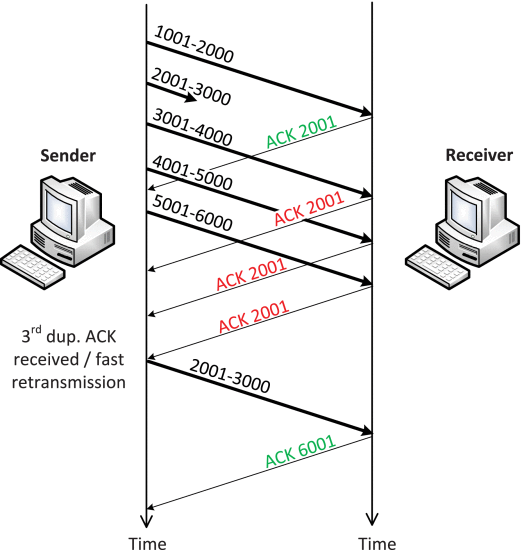
\includegraphics[height=5.5cm]{TCP_timeline}}
  \caption{A time-line of a \gls{TCP} interaction.}
  \label{fig:TCP_interaction}
\end{figure}
\end{itemize}

\section{\gls{IP}}
\begin{itemize}
\item Currently, coexist two different versions of the IP
  \cite{wikipedia_IP}:
  \begin{enumerate}
  \item \textbf{Version 4}: Defined in the 70's. Uses 32-bits IP addresses.
  \item \textbf{Version 6}: Defined in the 90's. Uses 128-bits IP addresses.
  \end{enumerate}
\item Responsible for the (\popup{``best effort''}{IP is classified as
    an unreliable protocol because it does not solve the transmission
    errors.} delivery of data packets.
\item The length of the packets must be $<6$4 KB (including the header).
\end{itemize}

\section{Routers}
\begin{itemize} 
\item Routers use the IP headers to \popup{define ``on-the-fly'' the
    transmission path of each packet}{Each router is responsible for
    choosing which output link it will use to retransmit each packet
    that arrives.}. This behaviour is known as the \textbf{datagram
    transmission model}.
\begin{figure}[H]
  \vspace{1ex}
  \centering
  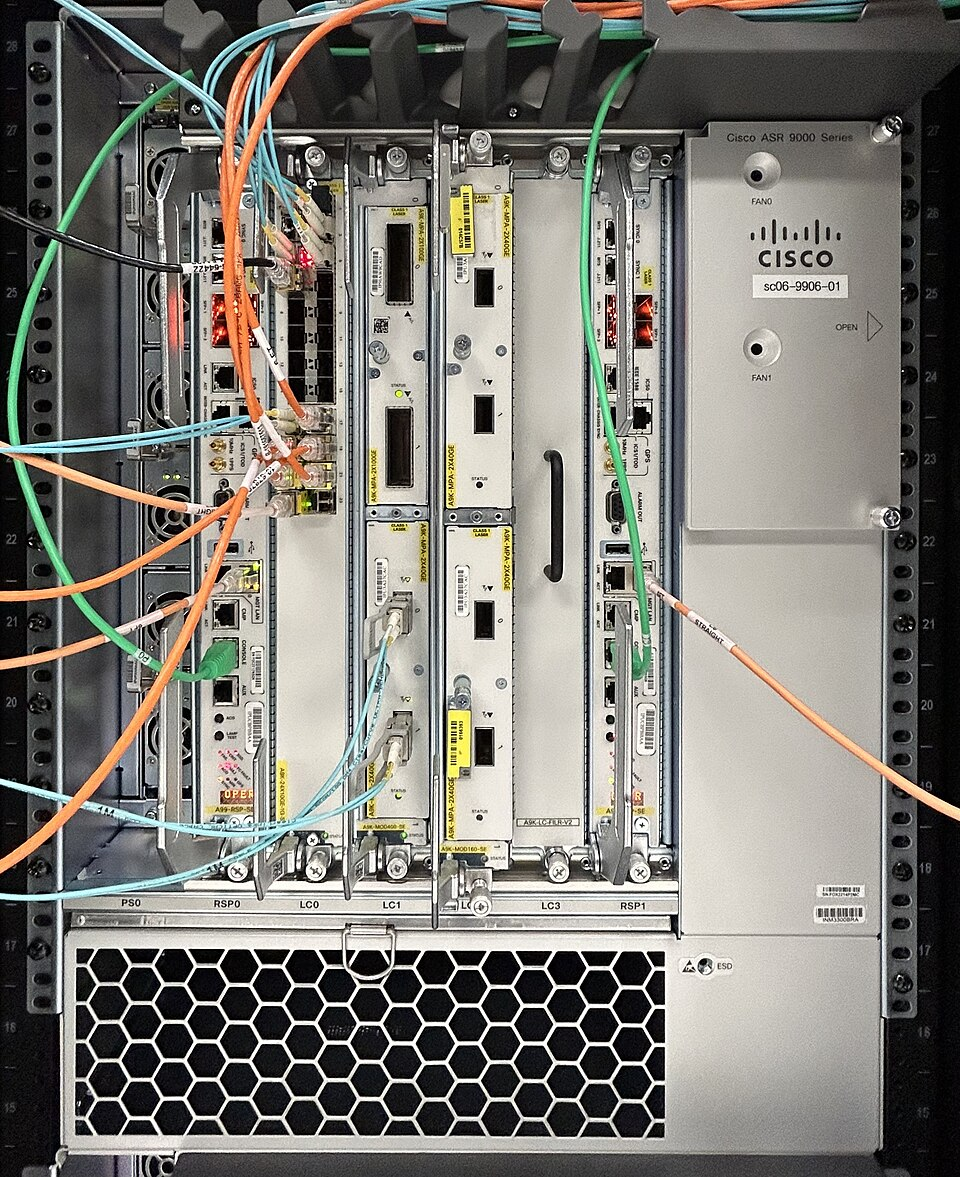
\includegraphics[height=0.65\textheight]{router}
  \caption{A router.}
  \label{fig:router}
\end{figure}
\end{itemize}

\section{Public and private IP addresses}
\begin{itemize}
\item Public IP addresses are used for public servers, such as the IP
  address of the Web server of the UAL.
\item Private IP addresses are used the rest of computers connected to
  the Internet. These addresses only are accesible from the local
  (private) network.
\item The router that interconnect a private network with the rest of
  the Internet is a \gls{NAT} device. All the private hosts use the
  public IP address of the \popup{NAT}{... device. It is common to say
    only ``NAT'' instead of ``NAT device'' or ``NAT box''}.
\end{itemize}

